\documentclass{beamer}

\title{Final Results}   
\subtitle{TCP PhD School}
\author{Team SaRoLa - Saad, Robert, Lars} 
\date{\today}

\usepackage{tikz}
\usetikzlibrary{positioning,calc}

\begin{document}

\begin{frame}
  \titlepage
\end{frame}

\begin{frame}{Steps we took}
	\begin{itemize}
		\item Analyze examples
		\item Implement tasks in thyroid example
		\item Removed dynamic memory allocation and moved FANN to FRAM
		\item Optimized NN (less neurons in hidden layer)
	\end{itemize}
\end{frame}

\begin{frame}{Implementation -- Architecture}
\centering
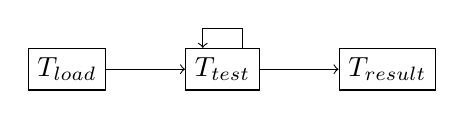
\begin{tikzpicture}
\node[draw,rectangle] (task-load) {$T_{load}$};
\node[draw,rectangle,right=of task-load] (task-test) {$T_{test}$};
\node[draw,rectangle,right=of task-test] (task-result) {$T_{result}$};

\draw[->] (task-load) -- (task-test);
\draw[->] (task-test) -- (task-result);
\draw[->] ($(task-test.north)+(0.25,0)$) -- ++(0,0.25cm) -- ++(-0.5,0) -- ++(0,-0.25);
\end{tikzpicture}

\begin{itemize}
	\item \textbf{$T_{load}$} Initialize FANN
	\item \textbf{$T_{test}$} Runs a single test
	\item \textbf{$T_{result}$} Print results and while(1);
\end{itemize}
\end{frame}

\begin{frame}{Optimization}
	\centering
	\begin{itemize}
		\item Reduce number of neurons in hidden layer
	\end{itemize}
	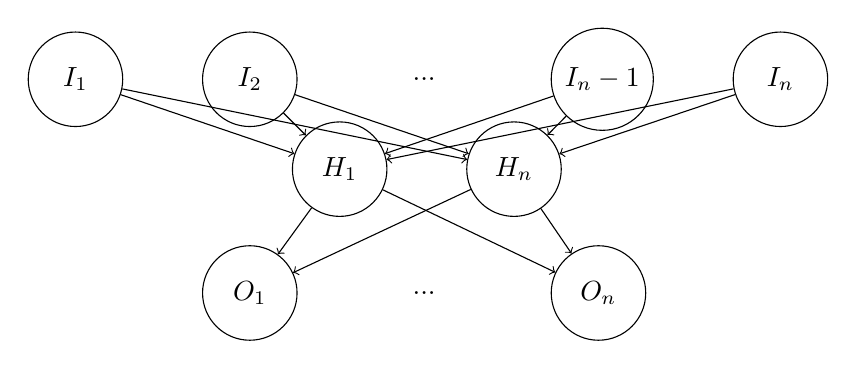
\begin{tikzpicture}[minimum width=1.2cm]
		\node[draw,circle] (i1) {$I_1$};
		\node[draw,circle,right=of i1] (i2) {$I_2$};
		\node[circle,right=of i2] (ip) {...};
		\node[draw,circle,right=of ip] (in1) {$I_n - 1$};
		\node[draw,circle,right=of in1] (in) {$I_n$};
		
		\node[draw,circle,below right=.4cm of i2] (h1) {$H_1$}; 
		%\node[circle,right=of h1] (hp) {...}; 
		\node[draw,circle,right=of h1] (hn) {$H_n$};
		
		\node[draw,circle,below=1.5cm of i2] (o1) {$O_1$}; 
		\node[circle,right=of o1] (op) {...}; 
		\node[draw,circle,right=of op] (on) {$O_n$}; 
		
		\draw[->] (i1) -- (h1);
		\draw[->] (i2) -- (h1);
		\draw[->] (in1) -- (h1);
		\draw[->] (in) -- (h1);
		
		\draw[->] (i1) -- (hn);
		\draw[->] (i2) -- (hn);
		\draw[->] (in1) -- (hn);
		\draw[->] (in) -- (hn);
		
		\draw[->] (h1) -- (o1);
		\draw[->] (hn) -- (o1);
		
		\draw[->] (h1) -- (on);
		\draw[->] (hn) -- (on);
	\end{tikzpicture}
\end{frame}

\end{document}